\documentclass[tikz]{standalone}

\usetikzlibrary{calc,positioning,shapes.geometric,backgrounds,fit,shadows.blur,arrows,arrows.meta,decorations.markings}

\newcommand*{\StrikeThruDistance}{0.15cm}%
\newcommand*{\StrikeThru}{\StrikeThruDistance,\StrikeThruDistance}%

\tikzset{strike thru arrow/.style={
    decoration={markings, mark=at position 0.5 with {
        \draw [blue, thick,-] 
            ++ (-\StrikeThruDistance,-\StrikeThruDistance) 
            -- ( \StrikeThruDistance, \StrikeThruDistance);}
    },
    postaction={decorate},
}}

\begin{document}
    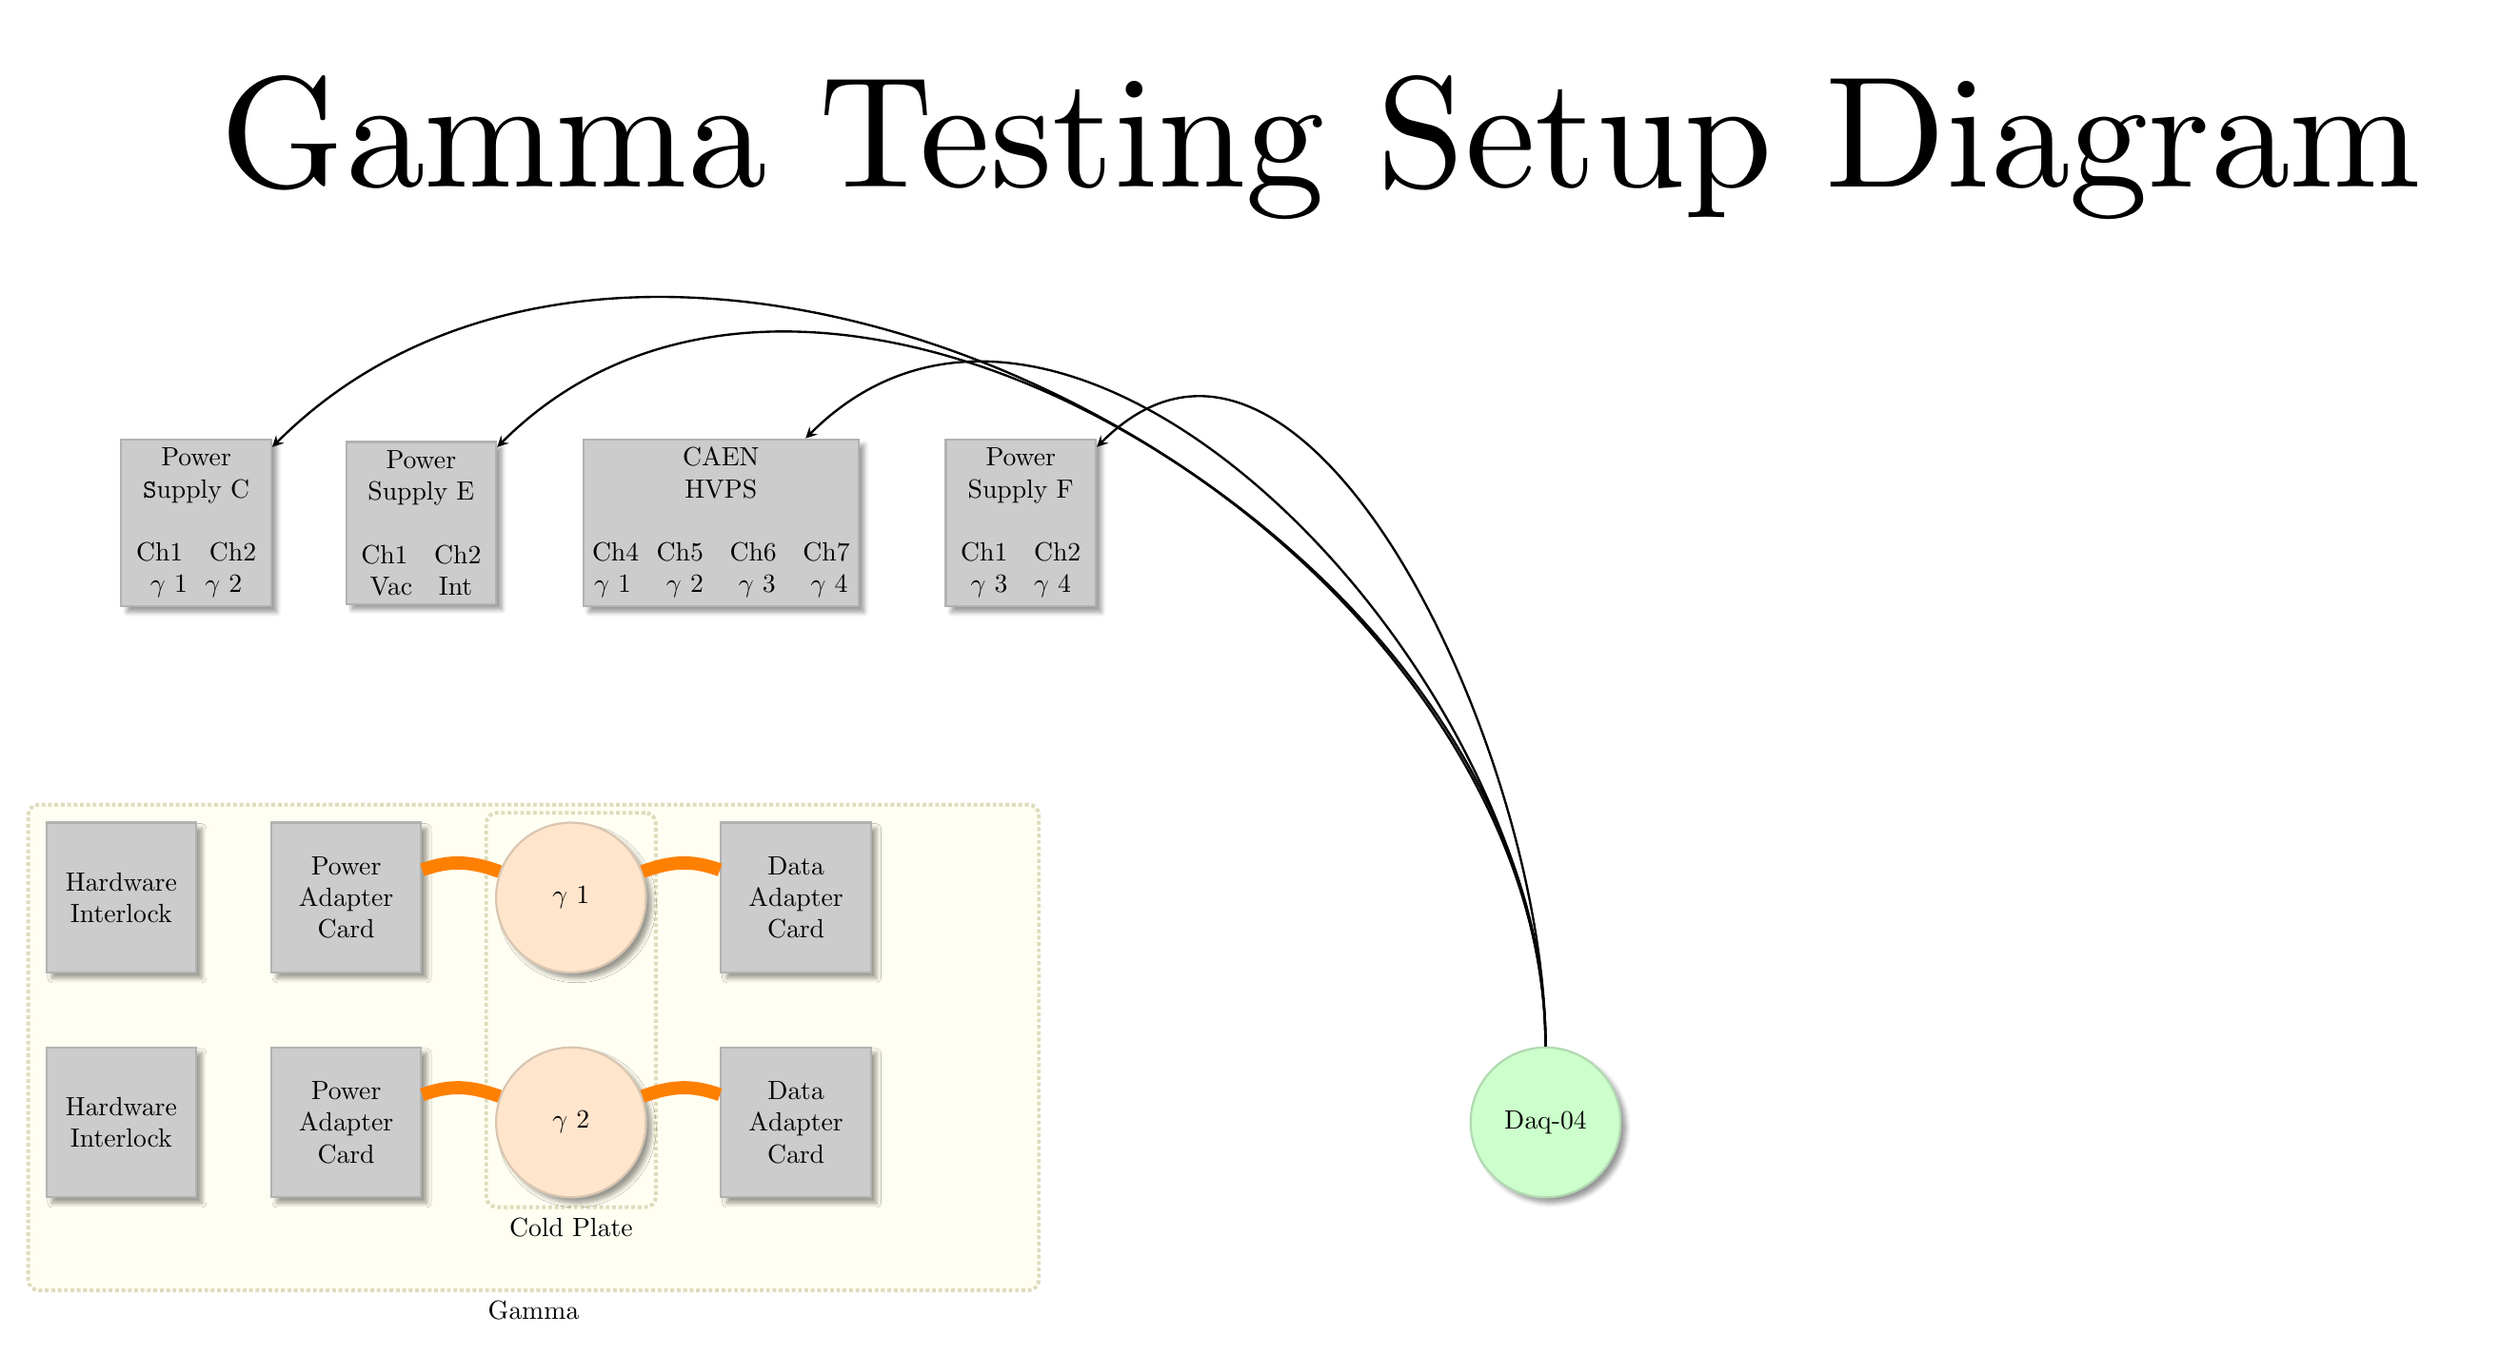
\begin{tikzpicture}[
	align=center,
        >=stealth,
        node distance=3cm,
	auto,
	line width=0.3mm,
        colorit/.style={
      	draw=#1!50!black!30,
      	fill=#1!20,
      	thick,
		blur shadow={shadow blur steps=5}
        },
        colorit/.default=black,
        database/.style={square, colorit=grey, shape border rotate=90, aspect=0.25, minimum size=2cm},
        software/.style={circle,colorit=green, minimum size=2cm},
	hardware/.style={rectangle,colorit=black, minimum size=2cm},
	module/.style={circle,colorit=orange, minimum size=2cm},
	database/.style={diamond,colorit=purple, minimum size=2cm},
	boxit/.style={
    	draw=#1!50!black!30,
		fill=#1!5,
		densely dotted,
		line width=0.5mm,
		rounded corners
	},
	boxit/.default=yellow
  	]
    % gamma
    \begin{scope}[every node/.append style={scale=6}, node distance=2.5cm]
        \node at (20,10) {Gamma Testing Setup Diagram};
    \end{scope}
    % power supplies
    \node[hardware] at (5,5) (psc) {Power\\\texttt Supply C\\\texttt {}\\\texttt {}Ch1 { { }}Ch2\\\texttt{}$\gamma$ 1 { }$\gamma$ 2};
    \node[hardware, right of = psc] (pse) {Power\\\texttt {}Supply E\\\texttt{}\\\texttt {}Ch1 { { }}Ch2\\\texttt{}Vac{ { { }}}Int};
    \node[hardware] at (12,5) (hvps) {CAEN\\\texttt {}HVPS\\\texttt {}\\\texttt {}Ch4{ { }}Ch5 { { }}Ch6 { { }}Ch7\\\texttt{}$\gamma$ 1 { { }} $\gamma$ 2 { { }} $\gamma$ 3 { { }} $\gamma$ 4 };
    \node[hardware] at (16,5) (psf) {Power\\\texttt {}Supply F\\\texttt {}\\\texttt {}Ch1 { { }}Ch2\\\texttt{}$\gamma$ 3 { } $\gamma$ 4};
    \node[software] at (23,-3) (daq) {Daq-04}
    edge[->, in = 45, out = 90] (psc)
    edge[->, in = 45, out = 90] (pse)
    edge[->, in = 45, out = 90] (hvps)
    edge[->, in = 45, out = 90] (psf);

    % test stand
    % gamma1
    \node[hardware] at (4,0) (int1) {Hardware\\Interlock}; 
    \node[hardware, right of = int1] (pac1) {Power\\Adapter\\Card};
    \node[module, right of = pac1] (gamma1) {$\gamma$ 1}
    edge[-,orange,line width=5,in=20,out=160] (pac1);
    \node[hardware,right of = gamma1] (dac1) {Data\\Adapter\\Card}
    edge[-,orange,line width=5,in=20,out=160] (gamma1);
    % gamma2
    \node[hardware] at (4,-3) (int2) {Hardware\\Interlock}; 
    \node[hardware, right of = int2] (pac2) {Power\\Adapter\\Card};
    \node[module, right of = pac2] (gamma2) {$\gamma$ 2}
    edge[-,orange,line width=5,in=20,out=160] (pac2);
    \node[hardware,right of = gamma2] (dac2) {Data\\Adapter\\Card}
    edge[-,orange,line width=5,in=20,out=160] (gamma2);

    % coldplate
    \begin{scope}[on background layer]
    \node[] at (3,1) (tl) {};
    \node[] at (16,-5) (br) {};
    \node [label=below:Gamma, boxit, fit=(tl)(br)]{};
    \node [label=below:Cold Plate, boxit, fit=(gamma1) (gamma2)] {};
    \end{scope}
    
\end{tikzpicture}
\end{document}
